%\title{LaTeX Portrait Poster Template}
%%%%%%%%%%%%%%%%%%%%%%%%%%%%%%%%%%%%%%%%%
% a0poster Portrait Poster
% LaTeX Template
% Version 1.0 (22/06/13)
%
% The a0poster class was created by:
% Gerlinde Kettl and Matthias Weiser (tex@kettl.de)
% 
% This template has been downloaded from:
% http://www.LaTeXTemplates.com
%
% License:
% CC BY-NC-SA 3.0 (http://creativecommons.org/licenses/by-nc-sa/3.0/)
%
%%%%%%%%%%%%%%%%%%%%%%%%%%%%%%%%%%%%%%%%%

%----------------------------------------------------------------------------------------
%	PACKAGES AND OTHER DOCUMENT CONFIGURATIONS
%----------------------------------------------------------------------------------------

\documentclass[a0,landscape]{a0poster}

\usepackage{multicol} % This is so we can have multiple columns of text side-by-side
\columnsep=100pt % This is the amount of white space between the columns in the poster
\columnseprule=3pt % This is the thickness of the black line between the columns in the poster

\usepackage[svgnames]{xcolor} % Specify colors by their 'svgnames', for a full list of all colors available see here: http://www.latextemplates.com/svgnames-colors

\usepackage{times} % Use the times font
%\usepackage{palatino} % Uncomment to use the Palatino font

\usepackage{graphicx} % Required for including images
\graphicspath{{figures/}} % Location of the graphics files
\usepackage[font=small,labelfont=bf]{caption} % Required for specifying captions to tables and figures
\usepackage{amsfonts, amsmath, amsthm, amssymb} % For math fonts, symbols and environments
\usepackage{wrapfig} % Allows wrapping text around tables and figures
\usepackage{indentfirst}

\usepackage[compact]{titlesec}
\titlespacing{\section}{0pt}{0pt}{10pt}
\titlespacing{\subsection}{0pt}{*0}{*0}
\titlespacing{\subsubsection}{0pt}{*0}{*0}

\setlength{\parskip}{10pt}
\setlength{\parsep}{0pt}
\setlength{\headsep}{0pt}
\setlength{\topskip}{0pt}
\setlength{\topmargin}{0pt}
\setlength{\topsep}{0pt}
\setlength{\partopsep}{0pt}

\begin{document}

%----------------------------------------------------------------------------------------
%	POSTER HEADER 
%----------------------------------------------------------------------------------------

% The header is divided into two boxes:
% The first is 75% wide and houses the title, subtitle, names, university/organization and contact information
% The second is 25% wide and houses a logo for your university/organization or a photo of you
% The widths of these boxes can be easily edited to accommodate your content as you see fit

\begin{minipage}[b]{0.78\linewidth}
\VeryHuge \color{NavyBlue} \textbf{HITRAN Application Programming Interface and Efficient Spectroscopic Tools (HAPIEST)}\\[0.1cm]% Title
\color{Black}\LARGE\textit{A GUI application for HAPI}\\[1.5cm] % Subtitle
\LARGE\textbf{\underline{J. Karns}$^a$$^,$$^b$, \underline{W. N. Matt}$^a$$^,$$^b$, \underline{R. V. Kochanov}$^b$$^,$$^c$, \underline{I.~E. Gordon}$^b$, \underline{L. S. Rothman}$^b$, \underline{Y. Tan}$^b$, R. Hashemi$^b$$^,$$^d$, S.~Kanbur$^a$, B. Tenbergen$^a$}\\[0.5cm] % Author(s)
\large $^a$\textit{State University of New York at Oswego, Oswego, NY, USA}
\large $^b$\textit{Atomic and Molecular Physics, Harvard-Smithsonian Center for Astrophysics, Cambridge, MA, USA}
\large $^c$\textit{Tomsk State University, Laboratory of Quantum Mechanics of Molecules and Radiative Processes, Tomsk, Russia}
\large $^d$\textit{University of Lethbridge, Alberta, Canada}
%\newline\Large \texttt{CONTACT INFO}\\
\end{minipage}
%
\begin{minipage}[b]{0.18\linewidth}
\begin{center}

\includegraphics[width=6cm]{OswegoLogo}\

\includegraphics[width=4cm]{HitranLogo}\

\includegraphics[width=4cm]{LethbridgeLogo}\

\includegraphics[width=5cm]{TomskLogo}\
\begin{minipage}{0.5\linewidth}\centering
Test out HAPIEST for\\
yourself and follow the development here.
\end{minipage}
\hfill
\begin{minipage}{.45\linewidth}

\includegraphics[width=10cm]{hapiest}\
\end{minipage}
\end{center}

\end{minipage}

%\vspace{1cm} % A bit of extra whitespace between the header and poster content

%----------------------------------------------------------------------------------------

\begin{multicols}{3} % This is how many columns your poster will be broken into, a portrait poster is generally split into 2 columns

%----------------------------------------------------------------------------------------
%	INTRODUCTION
%----------------------------------------------------------------------------------------

\color{Black}
\section*{\underline{Introduction}}
The goal of HAPIEST is to simplify the use of the HITRAN Application Programming Interface (HAPI) for all users. Currently, HAPI requires some knowledge of Python and use of the command line. HAPIEST should retain as much of the funtionality HAPI as is possible in a simple GUI, while making it easier to access and use for the user. HAPIEST currently allows users the capability to fetch/download and locally store data from the HITRAN database, edit local data, and also to generate and plot spectral functions. In it's current form, HAPIEST is split up into 3 windows, one window for data management and editing, and two windows for graphing/graph display.

%----------------------------------------------------------------------------------------
%	WINDOWS
%----------------------------------------------------------------------------------------

\section*{\underline{Data Management}}

\subsection*{Fetch Tab}
The Fetch tab allows the user to download data from HITRAN onto their local disk for the available molecules and their supported isotopologues. Further, the user can select from the \textit{Parameter Groups} list and \textit{Parameters} list to download more specific data. This window is the users primary method of obtaining data.
\begin{center}
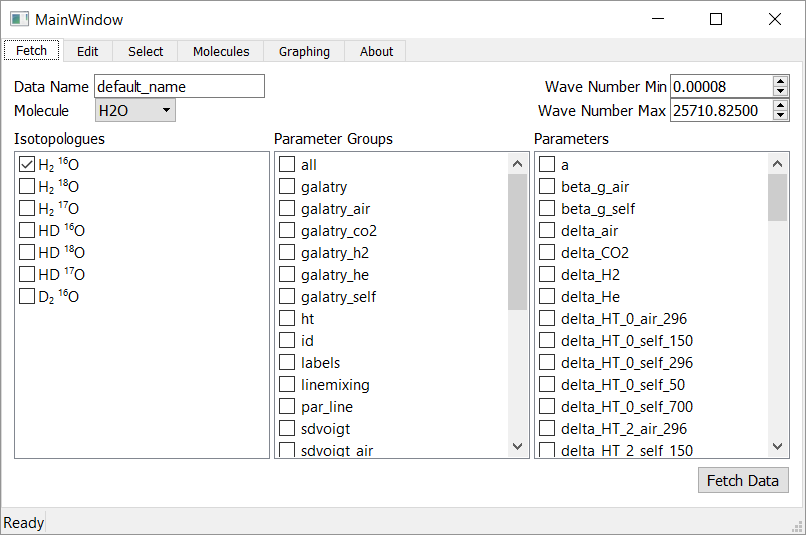
\includegraphics[scale = 1.5]{MainWindow_Fetch.png}
\end{center}
%\subsection*{Select Tab}
%Select-
%\begin{center}
%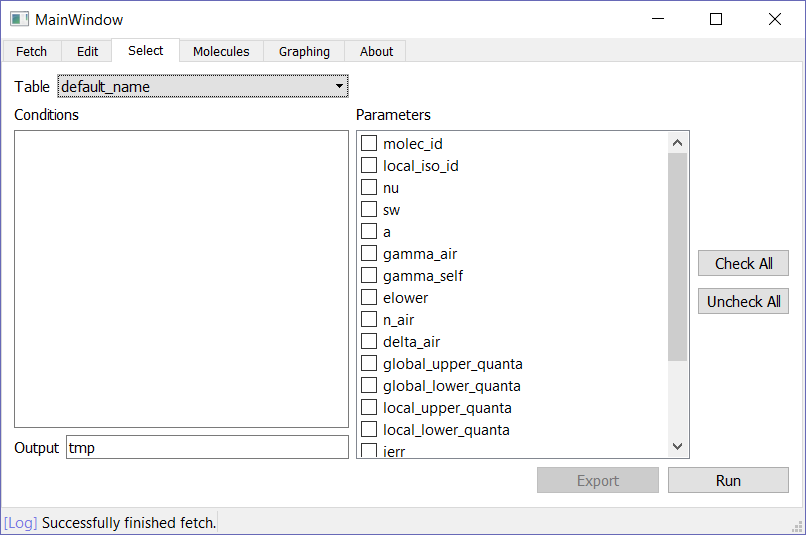
\includegraphics[scale = 1.5]{MainWindow_Select.png}
%\end{center}
\subsection*{Edit Tab}
The Edit tab allows users to view and edit local data that they have downloaded using HAPI/HAPIEST.
\begin{center}
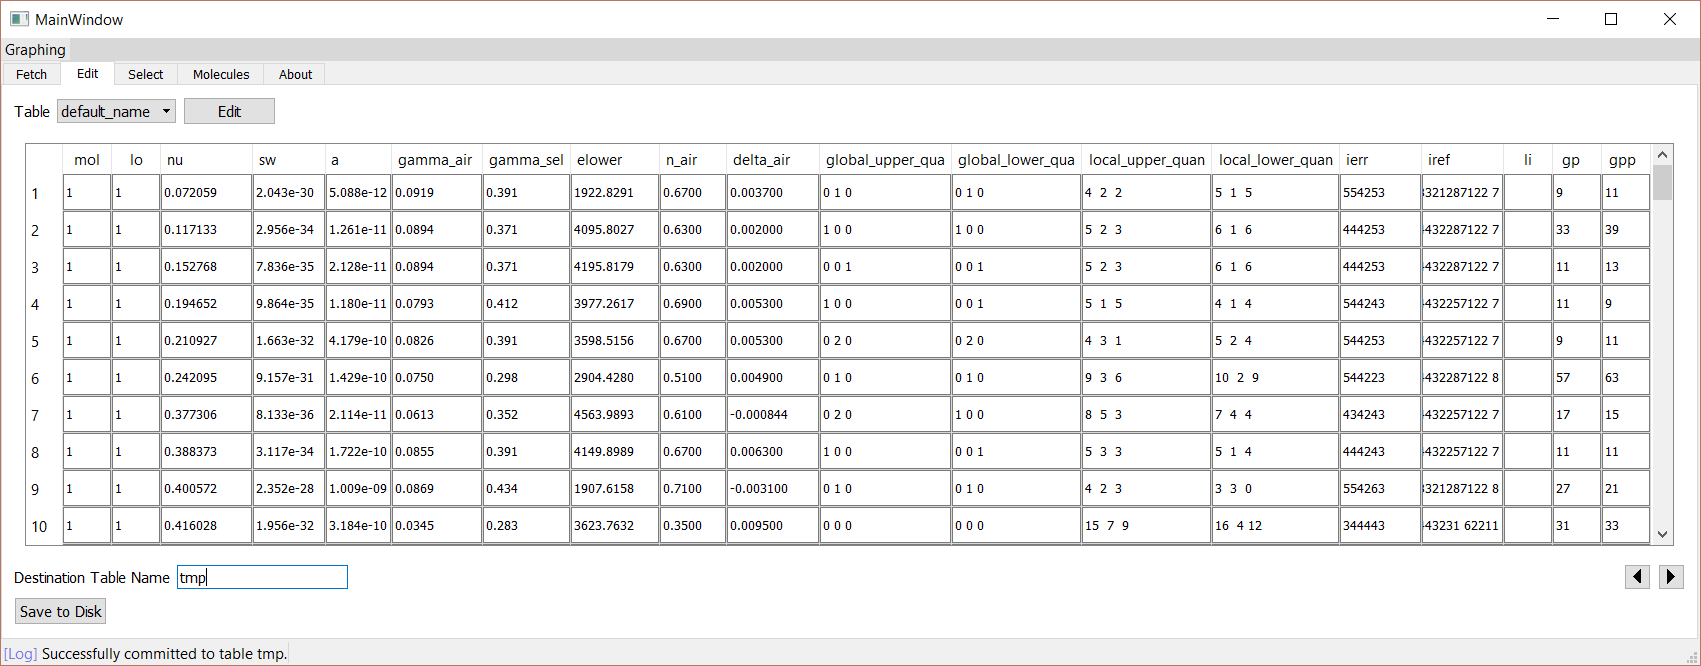
\includegraphics[scale = 1]{MainWindow_Edit.png}
\end{center}
\vfill\null
\columnbreak
\subsection*{Molecule Tab}
The Molecule tab provides users with information about available molecules (currently does not support isotopologues) including and image of the chemical makeup, and unique identifiers to aid further inquiry.
\begin{center}
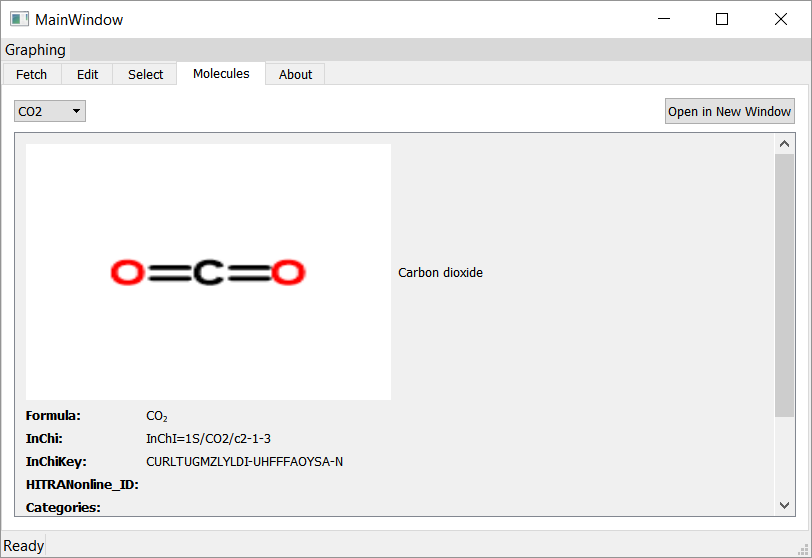
\includegraphics[scale = 1.5]{MainWindow_Molecules.png}
\end{center}

\section*{\underline{Graphing}}
\subsection*{Creating Graphs}
In the Graphing tab, the user is given a list of parameter fields that they may populate in order create the specific graph they need for each graph type (Absorption Coefficient; Absorption, Transmittance, and Radiance Spectra graphs). Multiple plots of the same type may be graphed together.
\begin{center}
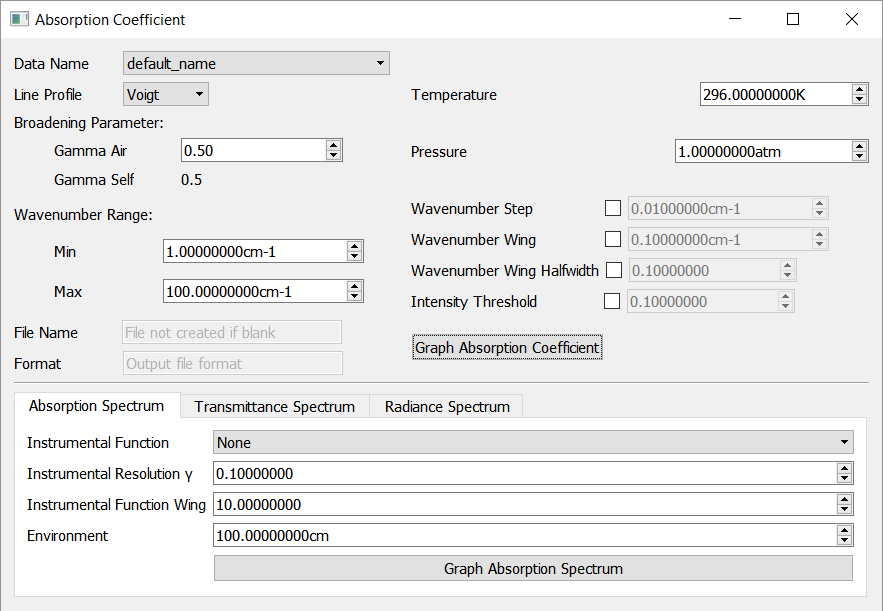
\includegraphics[scale = 1.5]{GraphingWindow.png}
\end{center}
\vfill\null
\columnbreak
\subsection*{Displaying Graphs}
The graph produced in the Graphing tab is displayed in a new window. This window provides the user tools to view and save graphs to local disk. Current functionality allows the user to zoom in on graphs, and will soon provide additional analysis tools and the ability to download graphs in popular image formats. 
\begin{center}
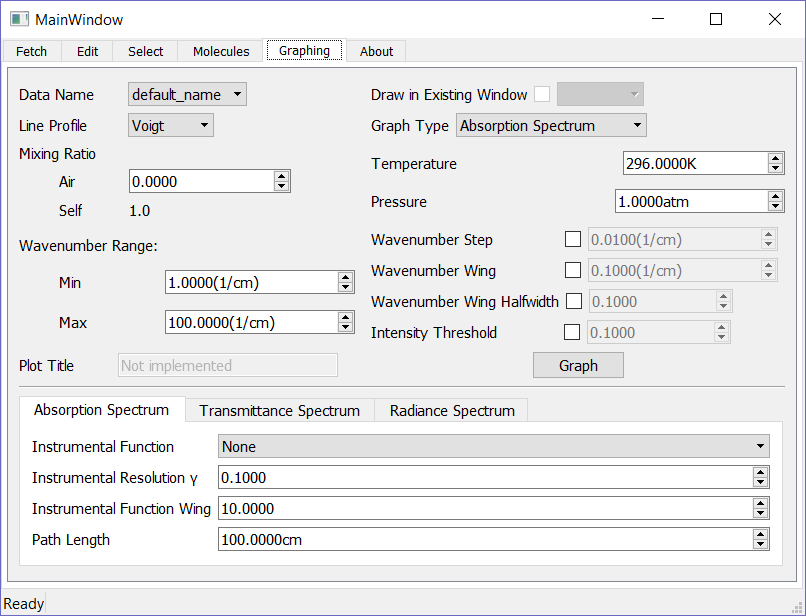
\includegraphics[scale = 1.5]{MainWindow_Graphing.png}
\end{center}
\begin{center}
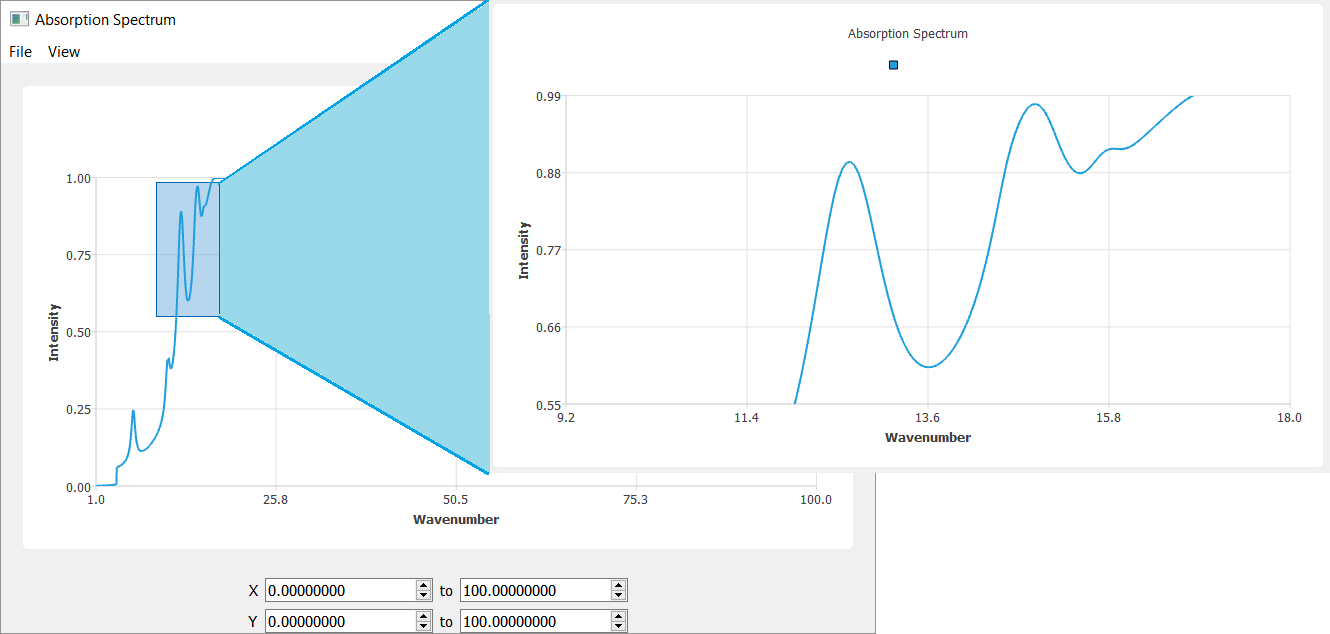
\includegraphics[scale = 1.2]{GraphDisplayWindow_ZoomDemo.png}
\end{center}
%----------------------------------------------------------------------------------------
%	CONCLUSIONS
%----------------------------------------------------------------------------------------

\section*{\underline{Summary}}
HAPIEST is an application built to provide a wider audience with the basic functionality of HAPI, including data fetching and selecting, generation of graphs of the spectral functions, all while maintaining ease of use and cross-platform capabilities.

\section*{\underline{Current Forthcoming Features}}

\begin{itemize}
\item Download graphs in popular image formats
\item Compatibility with HAPI 2.0
\item Update visual elements
\item Auto-Generate list of data sources
\end{itemize}

%----------------------------------------------------------------------------------------
%	REFERENCES
%----------------------------------------------------------------------------------------

%\nocite{*} % Print all references regardless of whether they were cited in the poster or not
%\bibliographystyle{plain} % Plain referencing style
%\bibliography{sample} % Use the example bibliography file sample.bib

%----------------------------------------------------------------------------------------

\end{multicols}
\end{document}
